\documentclass{article}
\usepackage[utf8]{inputenc}
\usepackage{amsmath}
\usepackage{ifsym}
\usepackage{pythonhighlight}
\usepackage{graphicx}
\usepackage[a4paper, total={6in, 8in}]{geometry}

\usepackage{listings}
\usepackage{color}

\definecolor{dkgreen}{rgb}{0,0.6,0}
\definecolor{gray}{rgb}{0.5,0.5,0.5}
\definecolor{mauve}{rgb}{0.58,0,0.82}

\lstset{frame=tb,
  language=Java,
  aboveskip=3mm,
  belowskip=3mm,
  showstringspaces=false,
  columns=flexible,
  basicstyle={\small\ttfamily},
  numbers=none,
  numberstyle=\tiny\color{gray},
  keywordstyle=\color{blue},
  commentstyle=\color{dkgreen},
  stringstyle=\color{mauve},
  breaklines=true,
  breakatwhitespace=true,
  tabsize=3}
  
\title{Labwork 10 - Project on applying Kuwahara filter using Numba Cuda}
\author{Nguyen Le Tuan Duy - M21.ICT.004}
\date{}



\begin{document}

\maketitle
\section{Introduction and Theory}
In this final labwork, I implement the Kuwahara filter, a smoothing filter for image that preserve the edge in the image. For each pixel, the filter choosing the 4 different window, in 4 different side of the image. The window size is chosen based on user decision. For each side, the standard deviation of the V value in HSV color of the pixel is calculated. The side with the lowest standard deviation will be chosen to recreate the value of current pixel by averaging all the pixel value on the area of the window. 

In this project, I will try to compare the execution speed when implementing Kuwahara filter by CPU and by GPU using Numba Cuda in Python. Some comparison when choosing different block size of GPU is also considered.

\section{Image preparation}
Firstly, we need to load the image:
\begin{python}
img = Image.open('000054.JPG')
numpy_img = np.asarray(img)
numpy_img = numpy_img.astype('float64')
numpy_img = numpy_img/255


window_size = 4 #input the window side here
numpy_img = np.pad(numpy_img, [(window_size,window_size),(window_size,window_size),(0,0)])
\end{python}

In order to have the window in both 4 sides in the pixel that near the edge of the image, I have to pad the image with the size equal to window size. In here I pad the image with zero value.

\begin{figure}
    \begin{center}
        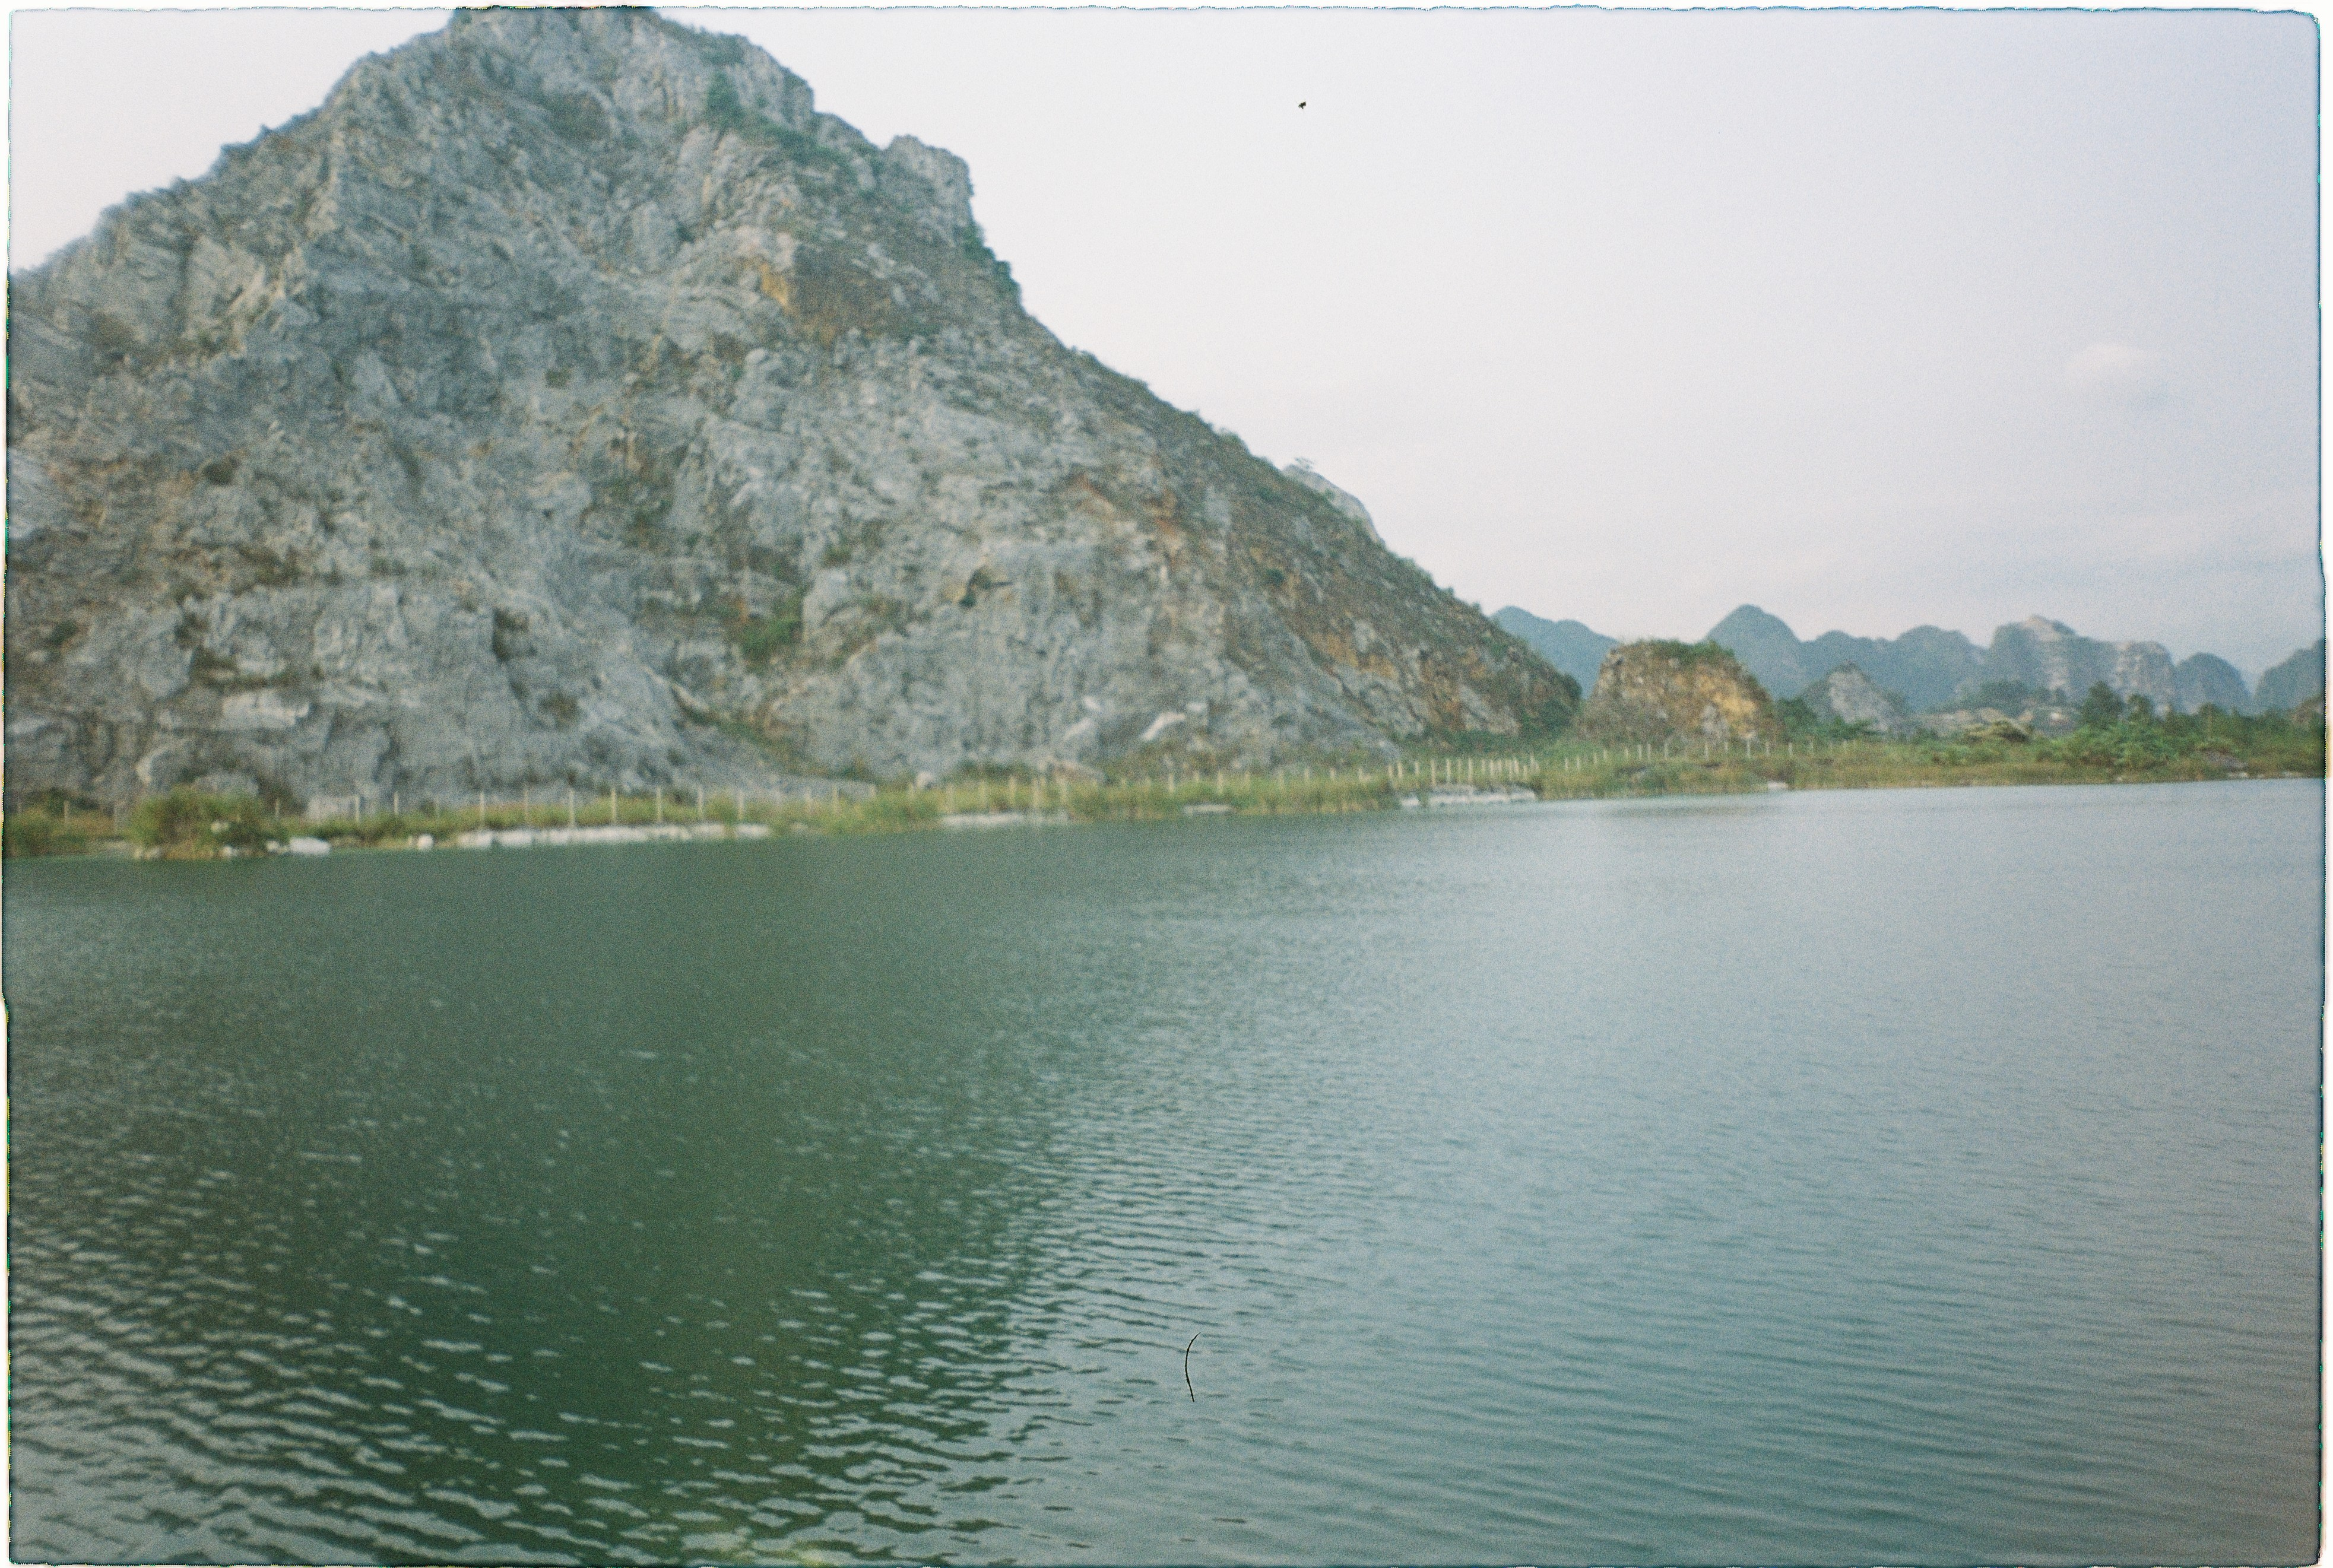
\includegraphics[scale=0.06]{000054.JPG}
        \caption{Original image}
    \end{center}
\end{figure}

Since Kuwahara filter also require the image in HSV color form, we need to have the HSV version of the image first. For this part, I reuse the implementation code from previous labwork using Numba:

\begin{python}
    @cuda.jit
def RGB2HSV(src, dst):
    tidx = cuda.threadIdx.x + cuda.blockIdx.x * cuda.blockDim.x
    tidy = cuda.threadIdx.y + cuda.blockIdx.y * cuda.blockDim.y
    max_ch = max(src[tidx, tidy, 0], src[tidx, tidy, 1], src[tidx, tidy, 2])
    min_ch = min(src[tidx, tidy, 0], src[tidx, tidy, 1], src[tidx, tidy, 2])
    delta = max_ch - min_ch

    if delta == 0:
        dst[0, tidx, tidy] = 0
    elif max_ch == src[tidx, tidy, 0]:
        dst[0, tidx, tidy] = 60 * (((src[tidx, tidy, 1]-src[tidx, tidy, 2])/delta) % 6)
    elif max_ch == src[tidx, tidy, 1]:
        dst[0, tidx, tidy] = 60 * (((src[tidx, tidy, 2]-src[tidx, tidy, 0])/delta)+2)
    elif max_ch == src[tidx, tidy, 2]:
        dst[0, tidx, tidy] = 60 * (((src[tidx, tidy, 0]-src[tidx, tidy, 1])/delta)+4)

    if max_ch == 0:
        dst[1, tidx, tidy] = 0
    else:
        dst[1, tidx, tidy] = delta/max_ch

    dst[2, tidx, tidy] = max_ch
\end{python}

\begin{python}
blocksize = (2,2)
gridSize = (math.ceil(width/blocksize[0]), math.ceil(height/blocksize[1]))
HSVOutput = cuda.device_array((3, width, height), np.float64)
devInput = cuda.to_device(numpy_img)
RGB2HSV[gridSize, blocksize](devInput, HSVOutput)
HSV_out = HSVOutput.copy_to_host()
\end{python}

\section{Kuwahara CPU}
For each pixel, not including the padded one, we create a list of range of 4 windows from 4 sides:
\begin{python}
    for x in range(w, img_RGB.shape[0]-w):
        for y in range(w,img_RGB.shape[1]-w):
            range_List = (((x-w, x+1), (y-w, y+1)),
                        ((x, x+w+1), (y-w, y+1)),
                        ((x-w, x+1), (y, y+w+1)),
                        ((x, x+w+1), (y, y+w+1)))
\end{python}

Next step, we compute the standard deviation of each window to chose the lowest one:
\begin{python}
            minid = 0
            minstd = 256

            for window in range(4):
                win_sum = 0

                for i in range(*range_List[window][0]):
                    for j in range(*range_List[window][1]):
                        win_sum += img_HSV[2, i, j]

                n = (w+1)**2
                winMean = win_sum/n
                win_sum = 0

                for i in range(*range_List[window][0]):
                    for j in range(*range_List[window][1]):
                        win_sum += (img_HSV[2, i, j] - winMean)**2 
                win_std = math.sqrt(win_sum/n)
                if win_std < minstd:
                    minstd = win_std
                    minid = window

            range_min = range_List[minid]
\end{python}

In here, when initialize the variable to store the min standard deviation, I set it to 256 cause the pixel value only range from 0 to 255, therefore the distance from any value to it mean cannot exceed this value. Calculating STD require two steps. The first step is to calculate the mean by take the sum of all and divide to the number of elements. The total of pixel in each window will be $(window\_size+1)^2 $. Then, we calculate the average square different of each value and the mean, and take the square root. Finaly, the id of the window that have lowest standard deviation is stored to calculate the average RGB value for the new current pixel value:

\begin{python}
                avg = 0
            for i in range(*range_min[0]):
                for j in range(*range_min[1]):
                    avg += img_RGB[i, j]
            finalrgb[x, y] = avg / (w+1)**2
    return finalrgb
\end{python}


\section{Kuwahara GPU}
In order to implement Numba Cuda for the Kuwahara filter, some step need to be modify.
Firstly, as usual, we need to initialize the BlockID in GPU:
\begin{python}
    tidx = cuda.threadIdx.x + cuda.blockIdx.x * cuda.blockDim.x
    tidy = cuda.threadIdx.y + cuda.blockIdx.y * cuda.blockDim.y
\end{python}
Instead of choosing the range to loop to avoid the padded part in the image, we need to specify the case of the blockID in the padded part of the image:

\begin{python}
        if tidx < w or tidx >= srcRGB.shape[0] - w or tidy < w or tidy >= srcRGB.shape[1] - w:
            dst[tidx, tidy, 0] = dst[tidx, tidy, 1] = dst[tidx, tidy, 2] = 0
            return
\end{python}
The other part is quite similar to those we did in CPU, exepct that we need to modify each R,G,B value separately to suitable with the way GPU manage the data:

\begin{python}
        minid = 0
    minstd = 256
    range_List = (((tidx-w, tidx+1), (tidy-w, tidy+1)),
                ((tidx, tidx+w+1), (tidy-w, tidy+1)),
                ((tidx-w, tidx+1), (tidy, tidy+w+1)),
                ((tidx, tidx+w+1), (tidy, tidy+w+1)))

    for window in range(4):
        win_sum = 0

        for i in range(*range_List[window][0]):
            for j in range(*range_List[window][1]):
                win_sum += srcHSV[2, i, j]

        n = (w+1)**2
        winMean = win_sum/n
        win_sum = 0

        for i in range(*range_List[window][0]):
            for j in range(*range_List[window][1]):
                win_sum += (srcHSV[2, i, j] - winMean)**2 
        win_std = math.sqrt(win_sum/n)
        if win_std < minstd:
            minstd = win_std
            minid = window

    range_min = range_List[minid]

    avg_r = 0
    avg_g = 0
    avg_b = 0
    for i in range(*range_min[0]):
        for j in range(*range_min[1]):
            avg_r += srcRGB[i, j, 0]
            avg_g += srcRGB[i, j, 1]
            avg_b += srcRGB[i, j, 2]

    dst[tidx, tidy, 0] = avg_r / (w+1)**2
    dst[tidx, tidy, 1] = avg_g / (w+1)**2
    dst[tidx, tidy, 2] = avg_b / (w+1)**2
\end{python}


Finally, we test the code with differents block size:

\begin{python}
blockSize_range = [(2,2),(4,4),(8,8),(16,16),(32,32)] #
for blockSize in blockSize_range:
  gridSize = (math.ceil(width/blockSize[0]), math.ceil(height/blockSize[1]))
  KuraOutput = cuda.device_array((numpy_img.shape), np.float64)
  devInput = cuda.to_device(numpy_img)
  time1 = time.time()

  KuwaharaGPU[gridSize, blockSize](devInput,HSVOutput, KuraOutput,window_size)
  imggpu = KuraOutput.copy_to_host()
  print('GPU time in seconds of blocksize ',blockSize,' : ', time.time()-time1)
\end{python}

\newpage
\section{Result and Discussion}
The table illustrate the result of time computing in CPU and in different block size of GPU. For the CPU, I have to resize the image 10 times and 5 times smaller for each dimension so that I can log the execution time on CPU, with the resize ratio, it can be estimated that the CPU take around 29 minutes (100 times compare to resize 10 times) for the original image.
\begin{table}[bp]
\caption{Times in different settings - Kuwahara filter }
\begin{tabular}{|c|c|c|c|c|c|c|c|c|}
\hline
\bfseries Type of running &CPU  &GPU2x2  &GPU4x4   &GPU8x8   &GPU16x16    &GPU32x32      \\
\hline\hline
\bfseries Resize 10 times     &17.46   &0.59 &0.004 &0.003 &0.003 &0.003    \\
\hline
\bfseries Resize 5 times     &70.42   &0.54 &0.014 &0.009 &0.0085 &0.009    \\
\hline
\bfseries Original     &est ~29m   &1.201 &0.19 &0.138 &0.099 &0.105    \\
\hline
\end{tabular}
\end{table} 

The result of the filter is quite similar between the CPU and GPU, and it also works well on the purpose of the smoothing filter. In here, I use the window size = 4 and it works quite noticeable with the resized image.
\begin{figure}
    \begin{center}
        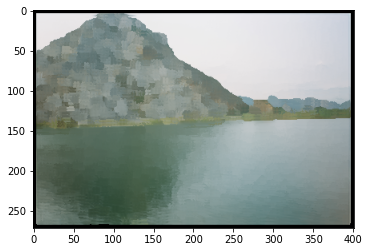
\includegraphics[scale = 0.5]{cpu-resize.png}
        \caption{CPU transformed image}
    \end{center}
\end{figure}

\begin{figure}
    \begin{center}
        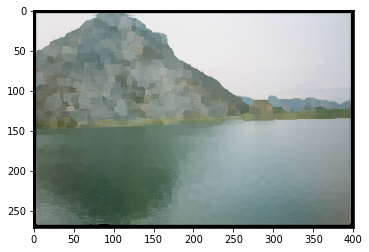
\includegraphics[scale = 0.5]{gpu-resize.png}
        \caption{GPU transformed image}
    \end{center}
\end{figure}

For the case of the original image using GPU, the different is harder to see if we still keep the window size = 4. if we increase the window size into 20, the image now is changing more significant. However, with large window size, the GPU(here is Tesla T4) will return memory allocation error with block size bigger than 4x4. The execution time for this case is also increase significantly, around 7 seconds


\begin{figure}
    \begin{center}
        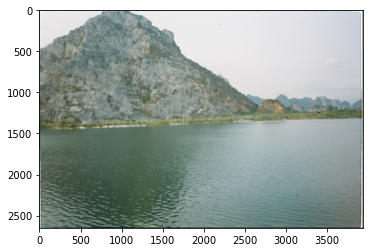
\includegraphics[scale = 0.5]{gpu - size3.png}
        \caption{Original size transformed image with window size = 4}
    \end{center}
\end{figure}


\begin{figure}
    \begin{center}
        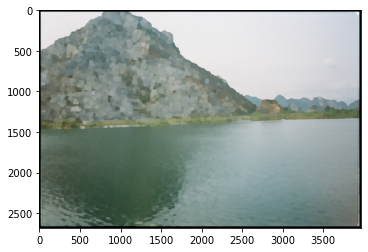
\includegraphics[scale = 0.5]{gpu-size20.png}
        \caption{Original size transformed image with window size = 20}
    \end{center}
\end{figure}







\end{document}